%-------------------------------------------------------------------------------
%							PREAMBULE
%-------------------------------------------------------------------------------

\documentclass[notes]{beamer}
% \documentclass[notes,handout,aspectratio=169]{beamer}   % Use this to print notes and disable animations

%%----------Color and design section ---------------------------

%%% Define colors and main theme-----


\useoutertheme{infolines}

% \usecolortheme{spruce}
% \useinnertheme{circles}

% \useoutertheme{shadow}

% \usetheme{JuanLesPins}
\usetheme{Antibes}
% \usetheme{Bergen}

\useoutertheme{smoothbars}
\colorlet{mygreen}{green!50!blue} 
\definecolor{navy}{rgb}{0.04706, 0.13725, 0.26667}

% \usecolortheme{whale}
\usecolortheme[named=navy]{structure}


% \useinnertheme[shadow]{rounded}
\setbeamertemplate{itemize items}{$\blacktriangleright$}  %% Triangles in itmize

\setbeamercolor{alerted text}{fg=violet}
\setbeamercolor{alerted text}{fg=red!90!black}


% \setbeamertemplate{enumerate items}[default]

\setbeamertemplate{navigation symbols}{}
%%----------------------------------------------------------------

\usepackage[fontsize=8]{scrextend} % Use this to force the fontsize

\usepackage{docmute} % To include multiple files

\usepackage{ragged2e}   %% For justification
\usepackage{etoolbox}
\usepackage{listings}

\usepackage{xcolor}
\usepackage{graphicx}
% \sethlcolor{mDarkTeal}
\graphicspath{ {./img/} }



%\usepackage{amsmath,bm,mathtools}
\usepackage{amsmath,mathtools}
% \usepackage[mathrm=sym]{unicode-math}
% \usepackage{bigints}
% \setmathfont{Fira Math Regular} 
% \setsansfont[BoldFont={Fira Sans SemiBold}]{Fira Sans Regular}

\usepackage[utf8]{inputenc}
\usepackage[T1]{fontenc}
\usepackage{textcomp}
\usepackage[sansmath]{libertinust1math}
% \usepackage{eulervm}

% \usepackage[font=small,textfont=it,justification=centering]{caption}
\usepackage[font={bf},justification=centering]{caption}
\usepackage{subcaption}
% \captionsetup{labelformat=empty,labelsep=none}    % Pour retirer le terme figure des titres
% \setbeamerfont{caption}{family=\sffamily,size=\small}

\usepackage{marvosym} %% For smileys

\usepackage{multirow}

\usepackage{cases} 
\usepackage{siunitx}

\usepackage{mathdots}

\usepackage[backend=bibtex,style=authoryear,maxnames=2,natbib=true]{biblatex} % Use the bibtex backend with the authoryear citation style (which resembles APA)
\addbibresource{bibliography.bib} % The filename of the bibliography
\usepackage[autostyle=true]{csquotes} % Required to generate language-dependent quotes in the bibliography 
\renewcommand*{\bibfont}{\scriptsize} % Pour reduire la taille des references

\usepackage{hyperref}     %% No coloring for hyperlinks, since links are everywhere
\usepackage{booktabs}

\usepackage{xparse}   %% To define new commands


\usepackage{cancel}   %% TO strikeout text


\usepackage[british]{babel}
\usepackage[useregional]{datetime2}

%-------------------------------------------------------------------------------
%							NEW COMMANDS
%-------------------------------------------------------------------------------


\newcommand{\tabhead}[1]{{\bfseries#1}}

%\newcommand{\bvec}[1]{\bm{\mathrm{#1}}}  %% Use this to make vectors
\newcommand{\bvec}[1]{\symbfup{#1}}  %% Use this to make vectors
%\newcommand{\bmat}[1]{\bm{\mathsf{#1}}}   %% Use this to make tensors/

\newcommand{\myvec}[2]{\begin{pmatrix} #1  \\ #2 \end{pmatrix}}   %% vecteur 2d
\newcommand{\mymat}[4]{\begin{pmatrix} #1 & #2 \\ #3 & #4 \end{pmatrix}}  %% Matrice 2*2

\apptocmd{\frame}{}{\justifying}{} % Allow optional arguments after frame.
% \addtobeamertemplate{block begin}{}{\justifying}  %new code

\newcommand{\zerodisplayskips}{%        %% To remove space after math box
  \setlength{\abovedisplayskip}{0pt}%
  \setlength{\belowdisplayskip}{0pt}%
  \setlength{\abovedisplayshortskip}{0pt}%
  \setlength{\belowdisplayshortskip}{0pt}}
% \appto{\normalsize}{\zerodisplayskips}
% \appto{\small}{\zerodisplayskips}
% \appto{\footnotesize}{\zerodisplayskips}

% \cols                                       %% Easy way to create columns with justifiable content
\newcommand{\mycols}[1]{%
  \begin{columns}[onlytextwidth]
    #1
  \end{columns}
}
% % % \col{size}{title}{content}                  %% Easy way to create columns with optional titles
\newcommand{\mycol}[2]{%
    \column{.#1\textwidth-.25cm}{%
        \parbox[t]{\columnwidth}{%
        #2}%
    }%
}


\newcommand{\myfig}[2]{
  \begin{figure}       
    \frame{\includegraphics[width=\textwidth]{#1}}       
    \caption*{\textcolor{green}{Figure:} #2.}
  \end{figure}
}


\newcommand{\mycap}[1]{\caption*{\textcolor{green}{Figure:} #1.}}
\newcommand{\mycaptab}[1]{\caption*{\textcolor{green}{Table:} #1.}}


%-------------------------------------------------------------------------------
%							TITLE PAGE
%-------------------------------------------------------------------------------
\begin{document}

% \setbeamercolor{postit}{fg=white,bg=mDarkTeal}

\title[Deep learning for inverse problems in radiative transfer]{Simulation of light propagation and reconstruction of a medium's density using deep neural networks}

% \institute[University of Strasbourg]{\small \textbf{ \hspace*{0.1mm} Referent teacher} \hspace*{11mm} \textbf{Supervisors} \\ \footnotesize Christophe PRUD'HOMME \hspace*{4mm} Michel DUPREZ \\ \hspace*{38mm} Stephane COTIN}
\institute[]{\small Sorbonne Université}


\author[Roussel Desmond Nzoyem]{\large \bfseries Roussel Desmond Nzoyem}

% \logo{
\includegraphics[width=0.6cm,height=1cm,keepaspectratio]{LogoBristol.png}}

\date[Soutenance mi-stage 2021]{\today}
% \date[Soutenance mi-stage]{\DTMdisplaydate{2021}{4}{20}{-1}}


\maketitle


%-------------------------------------------------------------------------------
%							INCLUDE THE CHAPTERS
%-------------------------------------------------------------------------------


\begin{frame}
  \small
  \frametitle{Contents}
  \tableofcontents
\end{frame}



%-------------------------------------------------------------------------------
%							FIRST SECTION
%-------------------------------------------------------------------------------

\section{\textsc{Introduction}}


\subsection{Test subsection title}


\begin{frame}[fragile,t]
  \frametitle{Motivation}
  
  \note{Floe: Un floe est un morceau de glace.}

  \mycols{

    \mycol{50}{
      \begin{exampleblock}{Enjeux écologiques}
        \begin{itemize}
          \item Etude climatique à échelle nature (SASIP)
          \item Prévisions climatiques avec précision
        \end{itemize}
      \end{exampleblock}

      \myfig{Ecological.jpg}{Prévision dans l'artique}
      }

    \pause

    \mycol{50}{
      \begin{alertblock}{Enjeux industrielles}
        \begin{itemize}
          \item Routes maritimes exploitables
          \item Comportemetn des stations offshores 
        \end{itemize}
      \end{alertblock}
      \myfig{IceRoutes.png}{Un navire dans la MIZ}

      }
  }
\end{frame}


\section{\textsc{Introduction2}}

\begin{frame}{Objectifs}

  \begin{definition}{Objectifs généraux}

    \begin{itemize}
      \item Modélisation et analyse mathématique de la notion de percussion
      \item Poursuite du développement d’un modèle de fracturation des floes
    \end{itemize}
  \end{definition}


  \begin{exampleblock}{Objectifs intermédiaires}

    \begin{enumerate}
      \item Lecture des travaux précédents:
      \begin{itemize}
        \item M. Rabatel, S. Labbé, et J. Weiss: Dynamics of an assembly of rigid ice floes (\citeyear{rabatel2015dynamics}); 
        \item Matthias Rabatel: Modélisation dynamique d’un assemblage de floes rigides (\citeyear{rabatel2015modelisation});
        \item Dimitri Balasoiu: Modélisation et simulation du comportement mécanique de floes de glace (\citeyear{balasoiu2020modelisation}).
      \end{itemize}
      
      \item Modélisation et simulation du deplacmeent des noeuds d'un floe isolé:
      \begin{itemize}
        \item en 1D;
        \item en 2D.
      \end{itemize}

      \item Introduction de la percussion dans le code préexistant.

    \end{enumerate}
  \end{exampleblock}

\end{frame}


% 
%-------------------------------------------------------------------------------
%							SECOND SECTION
%-------------------------------------------------------------------------------

\section{\textsc{État de l'art}}


\subsection{Thèse de M. Rabatel}


\begin{frame}{Cinétique du floe}
  \mycols{
    \mycol{50}{
      Les équations de Newton-Euler:
      \begin{align} \label{eq:neweu}
      \begin{dcases} 
        M_i \frac{\diff \dot{\bvec{G}}_i(t)}{\diff t} &= \bvec{F}_i, \\
        \mathcal{I}_i \frac{\diff \dot{\theta}_i(t)}{\diff t} &= \mathfrak{M}_i,
      \end{dcases}        
      \end{align}
      où pour le floe $i$ : 
      \begin{itemize}
        \item $M_i$ : masse du floe;
        \item $\bvec{F}_i$ : somme des forces par unité de volume;
        \item $\mathcal{I}_i$ : le moment d'inertie du floe $i$;
        \item $\mathfrak{M}_i$ : le moment dynamique en $G$.
      \end{itemize}
      Le système (\ref{eq:neweu}) se réécrit sous la forme :
      \begin{align*}    
          \mathcal{M}_i \frac{\diff W_i(t)}{\diff t} = \mathcal{H}_i(t) ,
      \end{align*}
      avec 
      \begin{align*}
      \mathcal{M}_i = 
      \begin{pmatrix}
          M_i & 0 & 0 \\ 0 & M_i & 0 \\ 0 & 0 & \mathcal{I}_i
      \end{pmatrix} , \quad
      W_i(t) = 
      \begin{pmatrix}
          \dot{\bvec{G}}(t) \\ \dot{\theta}_i(t)
      \end{pmatrix} , 
      \text{ et } \quad \mathcal{H}_i(t) = 
      \begin{pmatrix}
          \bvec{F}_i(t) \\ \mathfrak{M}_i(t)
      \end{pmatrix}.
      \end{align*}
    }


    \mycol{50}{
      \myfig{FloeRabatel}{Repères abosolu et local pour un floe \parencite{rabatel2015modelisation}}
    }
  }
  
\end{frame}



\begin{frame}{Interaction entre les floes}
  \mycols{

    \mycol{45}{
      \myfig{Collision1.png}{Interaction entre deux floes $\Omega_k$ et $\Omega_l$ au point $P_j$ \parencite{rabatel2015modelisation}}
    }

    \mycol{55}{Deux conditions à respecter:
    \begin{itemize}
      \item \alert{Condition unilatérale de Signorini} : afin de décrire la condition de non-interpénétration.
      \item \alert{Loi de friction de Coulomb} : afin de modéliser le comportement de friction pendant une collision.
    \end{itemize}}

    \note{Historiquement, on distingue ici deux approches:
    \begin{itemize}
      \item l'approche par régularisation: Hertz (force de contact proportionnelle à la distance d'inter-penetration); largement répandues en robotique, en VR, habits, etc...MAIS ON NE VEUT PAS D'INTERPÉNÉTRATION !
      \item l'approche non-régulière: développée par inclusion différentielle: efficace, mais difficile à manipuler. D'ou l'essort des méthodes LCP. 
    \end{itemize}}

  }

\end{frame}



\begin{frame}{Discussion sur la thèse}

  \mycols{

    \mycol{37}{
      \begin{itemize}
        \item Les floes sont rigides;
        \item Le modèle ne gère pas la rhéologie de la glace;
        \item Les coefficients de friction et de restitution sont limitants.
      \end{itemize}
    }

    \mycol{27}{
      \myfig{Derive.png}{Configuration initiale \parencite{rabatel2015modelisation}}
    }

    \mycol{32}{
      \begin{figure}[!h]
        \begin{subfigure}[b]{0.60\textwidth}
            \centering
            
\includegraphics[width=\textwidth]{DeriveBlock2.png}
            \caption{à 2h04}
        \end{subfigure}
        \begin{subfigure}[b]{0.60\textwidth}
            \centering
            
\includegraphics[width=\textwidth]{DeriveBlock3.png}
            \caption{à 3h40}
          \end{subfigure}
           \caption{Dérive sous l'effet de la force de Coriolis \parencite{rabatel2015modelisation}}
    \end{figure}

    }

  }

\end{frame}




\subsection{Thèse de D. Balasoiu}


\begin{frame}{Un modèle de fracture variationnel}
  L'énergie totale s'écrit :
  \begin{align*}
  \etot : \,\bigcup_{\sigma \in \Sigma } A_{\sigma} \times \left\{ \sigma \right\} &\rightarrow \mathbb{R} \\
  u &\mapsto \int_{\Omega \backslash \sigma} Ae(u) : e(u) \diff x + k\mathcal{H}^1(\sigma)\,,
  \end{align*}
  
  Une solution du problème de fracture fragile est un couple $(u^*, \sigma^*)$ qui vérifie:
  \vspace*{0.25cm}
  $$
  \etot(u^*,\sigma^*) = \min_{\sigma \in \Sigma}{\min_{u\in A_{\sigma}}{\etot(u,\sigma)}} \,.
  $$

	\note{$\Sigma$ c'est l'ensemble des fractures admissibles, et $A_{\sigma}$ l'ensemble des déplacements admissibles sur un floe qui présente déjà la fissure $\sigma$.}

  \myfig{PhaseField2.png}{Bifurcation d’une fracture \parencite{nagaraja2019phase}}

\end{frame}


\begin{frame}{Réseaux de ressorts régulier}

  \myfigsize{Ressort1.png}{Réseau de ressorts régulier \parencite{balasoiu2020modelisation}}{20}

  \vspace*{-0.25cm}
  \myfigsize{VoronoiDelaunay.png}{Tirage de points et diagrammes de Voronoi (à gauche) et Delaunay (à droite) \parencite{balasoiu2020modelisation}}{60}

  \note{Afin d'établir la condition de Dirichlet nécéssaire pour engendrer la fracture, on passe du modèle macroscopique à un modèle microscopique.}

\end{frame}


% 
%-------------------------------------------------------------------------------
%							THIRD SECTION
%-------------------------------------------------------------------------------



\section{\textsc{Travaux 1D}}


\subsection{Déplacement des n\oe{}uds}

\begin{frame}{Déplacement des noeuds d’un floe isolé (1)}

    \mycols{

        \mycol{50}{
            \myfigframe{Deplacement1D-Systeme.png}{Floe de glace 1D}

            \begin{figure}[!h]
                \begin{subfigure}[b]{0.47\textwidth}
                    \centering
                    \frame{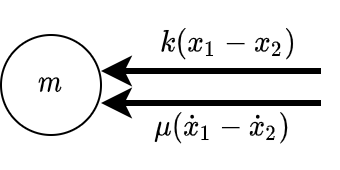
\includegraphics[width=\textwidth]{Deplacement1D-Masse1.png}}
                    % \caption{Sur la masse $m$ de gauche.}
                \end{subfigure}
                \begin{subfigure}[b]{0.43\textwidth}
                    \centering
                    \frame{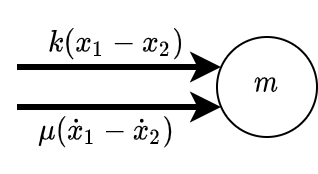
\includegraphics[width=\textwidth]{Deplacement1D-Masse2.png}}
                    % \caption{Sur la masse $m$ de droite.}
                \end{subfigure}
                   \caption{Bilan des forces}
            \end{figure}
        }
            \pause
        \mycol{50}{
            Les équations de Newton-Euler:
            \begin{align*}
                \begin{dcases}
                m\ddot x_1 = - k(x_1 - x_2) - \mu(\dot x_1 - \dot x_2) \,,\\
                    m \ddot x_2 =  k(x_1 - x_2) + \mu(\dot x_1 - \dot x_2) \,. 
                \end{dcases}
            \end{align*}

            On préfère la forme matricielle:
            \begingroup
            \color{red}
            \begin{align*}
                \begin{dcases}
                    \dot{Y}(t)= E Y(t) \,,\\
                    Y(0) = (0,0,v_0,-v'_0)^T \,,
                \end{dcases}
            \end{align*}
            \endgroup
            où :
            \begin{align*}
                E = \begin{pmatrix}
                    0 & 0 & 1 & 0 \\ 0 & 0& 0& 1 \\ -\frac{k}{m} & \frac{k}{m} & -\frac{\mu}{m} & \frac{\mu}{m} \\ \frac{k}{m} & -\frac{k}{m} & \frac{\mu}{m} & -\frac{\mu}{m}
                \end{pmatrix} \,,
                \text{ et } Y = \begin{pmatrix} x_1 \\ x_2 \\ \dot{x}_1 \\ \dot{x}_2 \end{pmatrix}.
            \end{align*}
        }
    }

    \note{Ici, ne pas utiliser un repère absolu, on peut utiliser un qui soit relatif au floe. Dans ce cas, on a convergence.}
    
\end{frame}


\begin{frame}[fragile]{Déplacement des noeuds d’un floe isolé (2)}

    % \begin{columns}[onlytextwidth]
		
	% 	\small
    %     \begin{column}{0.4\textwidth}
    %         \begin{lstlisting}[language=Python,captionpos=b,caption=Code de simulation]
    % Y0 = np.array([0,0, v0, -v_0])
    % t = np.linspace(0, tmax, N+1)
    % def model(Y, t):
    %     return E @ Y
    % Y = odeint(model, Y0, t)
    %         \end{lstlisting}
    %     \end{column}

	% 	\normalsize
    %     \mycol{60}{    
    %     \begin{exampleblock}{Théorème (Convergence du modèle 1D isolé)}
    %         Partant d'une position d'équilibre $x_1(0) = x_2(0) = 0$, les déplacements $x_1(\cdot)$ et $x_2(\cdot)$ des deux n\oe{}uds du floe 1D (avec viscosité $\mu > 0$) convergent  si et seulement si leurs vitesses initiales sont opposées, i.e. $\bvec v_0 = - \bvec v'_0$.
    %     \end{exampleblock}
    %     }
    % \end{columns}
    
    \large
    \begin{exampleblock}{Théorème (Convergence du modèle 1D à deux n\oe{}uds) \parencite{nzoyem2021thesis}}
        Partant d'une position d'équilibre $x_1(0) = x_2(0) = 0$, les déplacements $x_1(\cdot)$ et $x_2(\cdot)$ des deux n\oe{}uds du floe 1D (avec viscosité $\mu > 0$) convergent  si et seulement si leurs vitesses initiales sont opposées i.e. $\bvec v_0 = - \bvec v'_0$.
    \end{exampleblock}
    \normalsize
    En effet:
    \begin{align*}
        x_1(t) = \textcolor{myblack2}{\frac{t}{2}\left( v_0 - v'_0 \right)} + \frac{e^{\alpha t} \sin(\beta t)}{2\beta} \left( v_0 + v'_0 \right), \quad x_2(t) = \textcolor{myblack2}{\frac{t}{2}\left( v_0 - v'_0 \right)} - \frac{e^{\alpha t} \sin(\beta t)}{2\beta} \left( v_0 + v'_0 \right),
    \end{align*}
    où : $\alpha = -\frac{\mu}{m}$ et $\beta = -\frac{\sqrt{2km - \mu^2}}{m}$.
    \begin{figure}[!h]
        \centering
        \begin{subfigure}[t]{0.48\textwidth}
            \centering
            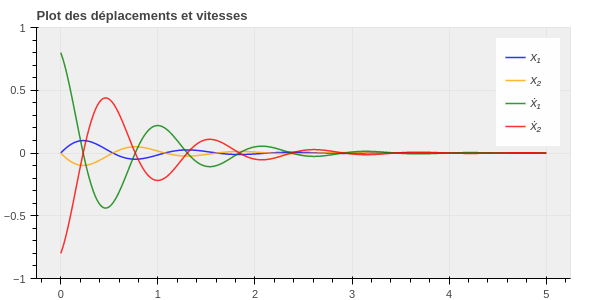
\includegraphics[width=\textwidth]{SimuDeplacement1D1.png}
            \caption{$v_0=v'_0 = 0.8$}
        \end{subfigure}
        \begin{subfigure}[t]{0.48\textwidth}
            \centering
            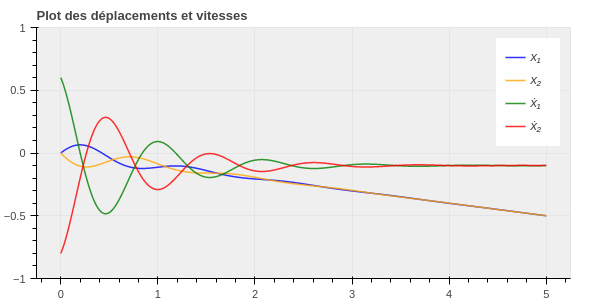
\includegraphics[width=\textwidth]{SimuDeplacement1D2.png}
            \caption{$v_0= 0.6$ et $v'_0 = 0.8$}
        \end{subfigure}    
        \caption{Simulation du déplacement d'un floe 1D à 2 n\oe{}uds}
    \end{figure}

    \note{Il faut absolument mentionner que la preuve graphique c'est la meilleure preuves de toutes :).}
    \normalsize

\end{frame}





\subsection{Percussion entre floes}



\begin{frame}{Collision parfaitement inélastique avec un floe encastré}

    \mycols{

        \mycol{55}{
            \myfigframe{Percussion1D-Systeme}{Collision 1D avec fixation d'un floe}

            \begin{figure}[!h]
                \begin{subfigure}[b]{0.54\textwidth}
                    \centering
                    \frame{
\includegraphics[width=\textwidth]{Percussion1D-Masse1}}
                \end{subfigure}
                \begin{subfigure}[b]{0.435\textwidth}
                    \centering
                    \frame{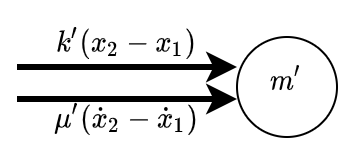
\includegraphics[width=\textwidth]{Percussion1D-Masse2}}
                \end{subfigure}
                   \caption{Bilan des forces}
            \end{figure}

            Le système est régi par les équations :
            \begin{align*}
                \begin{dcases}
                (m+m')\ddot x_1 = -kx_1 - \mu \dot x_1 + k'(x_2 - x_1) + \mu'(\dot x_2 - \dot x_1) \,, \\
                    m' \ddot x_2 =  -k'(x_2 - x_1) - \mu'(\dot x_2 - \dot x_1). 
                \end{dcases}
            \end{align*}

        }
        
        \pause
        \mycol{45}{

            \myfig{SimuPercussion1D.png}{Résultat de simulation}
        }

    }
    
\end{frame}


\begin{frame}{Collision parfaitement inélastique avec au départ un floe immobile}

    \mycols{

        \mycol{55}{
            \myfigframe{Percussion1D-Systeme-2}{Collision 1D sans mur}

            \begin{figure}[!h]
                \begin{subfigure}[b]{0.30\textwidth}
                    \centering
                    \frame{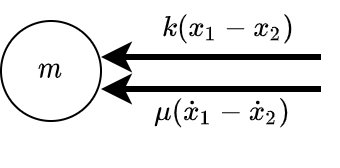
\includegraphics[width=\textwidth]{Percussion1D2-Masse1.png}}
                \end{subfigure}
                \begin{subfigure}[b]{0.38\textwidth}
                    \centering
                    \frame{
\includegraphics[width=\textwidth]{Percussion1D2-Masse2}}
                \end{subfigure}
                \begin{subfigure}[b]{0.26\textwidth}
                    \centering
                    \frame{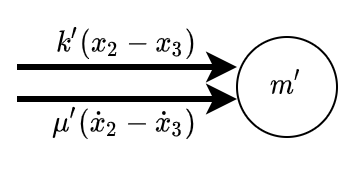
\includegraphics[width=\textwidth]{Percussion1D2-Masse3}}
                \end{subfigure}
                   \caption{Bilan des forces}
            \end{figure}

            Le système est régi par les équations :
            \begin{align*}
                \begin{dcases}
                m\ddot x_1 = -k(x_1 - x_2) - \mu (\dot x_1 - \dot x_2) \,, \\
                (m+m')\ddot x_2 = k(x_1 - x_2) + \mu (\dot x_1 - \dot x_2) - k'(x_2 - x_3) - \mu'(\dot x_2 - \dot x_3) \,, \\
                    m' \ddot x_3 =  k'(x_2 - x_3) + \mu'(\dot x_2 - \dot x_3) \,. 
                \end{dcases}
            \end{align*}

        }

        \pause
        \mycol{45}{
            % \myfig{SimuPercussion1D2.png}{Résultat de simulation}

            \vspace*{-0.25cm}

            \begin{figure}[!h]
                \begin{subfigure}[t]{\textwidth}
                    \centering
                    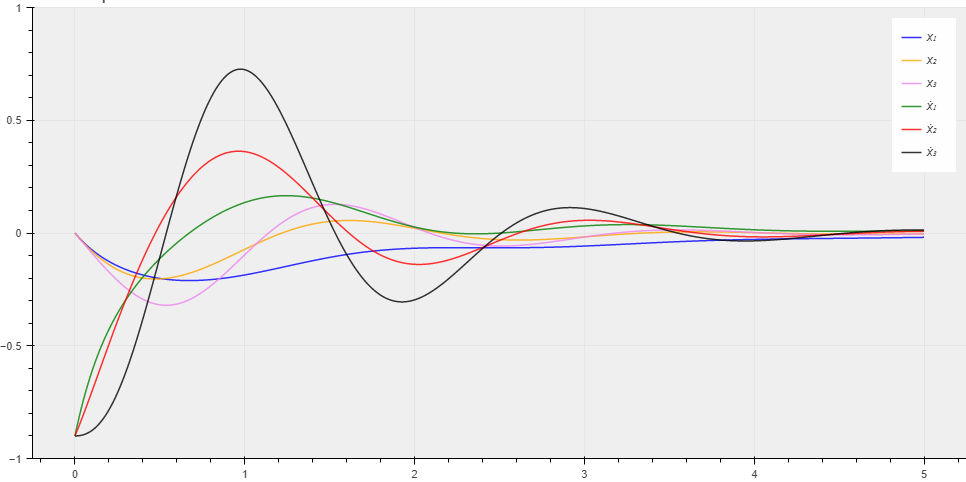
\includegraphics[width=0.9\textwidth]{SimuPercussion1D2.png}
                    \caption{Cas convergent}
                \end{subfigure}
                \begin{subfigure}[t]{\textwidth}
                    \centering
                    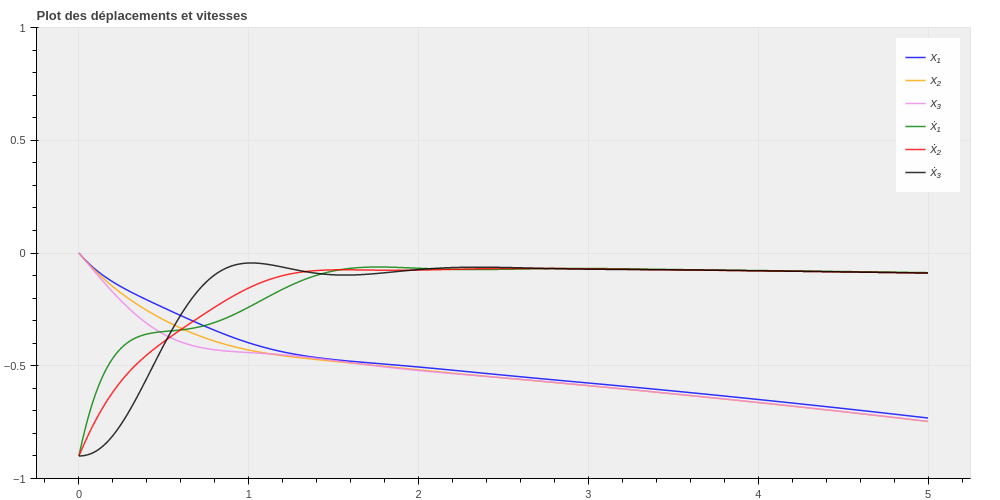
\includegraphics[width=0.9\textwidth]{SimuPercussion1D2NonConv.png}
                    \caption{Cas non convergent}
                \end{subfigure}
                %    \caption{Résultats de simulation}
            \end{figure}

            % \pause
            \vspace*{-0.1cm}
			\small
            % \begin{alertblock}{Note}
            %     Le critère de convergence n'est pas clair (i.e. $\mu << \mu'$, etc.)!
            % \end{alertblock}
            \begin{tcolorbox}[colback=red!5,colframe=red!50!black,arc=0mm,boxrule=0.1mm,title=Remarque]
                \vspace*{-0.1cm}
                    Le critère de convergence n'est pas clair (i.e. $\mu << \mu'$, $k$ très grand, etc.)!
                \vspace*{-0.1cm}
            \end{tcolorbox}
            \normalsize

        }

    }
    
\end{frame}


\begin{frame}{Collision inélastique avec séparation des masses}

    \mycols{

        \mycol{50}{
            \myfigframe{Percussion1D-Systeme-3}{Collision 1D inélastique}

            \vspace*{-0.5cm}
            \begin{figure}[!h]
                \begin{subfigure}[b]{0.35\textwidth}
                    \centering
                    \frame{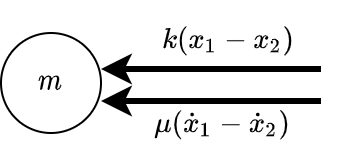
\includegraphics[width=\textwidth]{Percussion1D3-Masse1.png}}
                \end{subfigure}
            %     \hfill
                \begin{subfigure}[b]{0.48\textwidth}
                    \centering
                    \frame{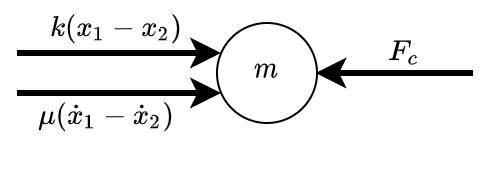
\includegraphics[width=\textwidth]{Percussion1D3-Masse2}}
                \end{subfigure}
            %     \hfill
                \begin{subfigure}[b]{0.44\textwidth}
                    \centering
                    \frame{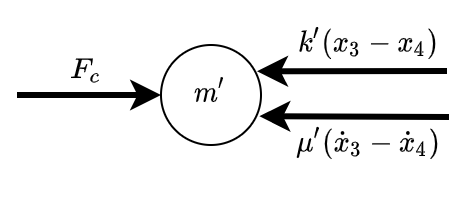
\includegraphics[width=\textwidth]{Percussion1D3-Masse3}}
                \end{subfigure}
            %     \hfill
                \begin{subfigure}[b]{0.35\textwidth}
                    \centering
                    \frame{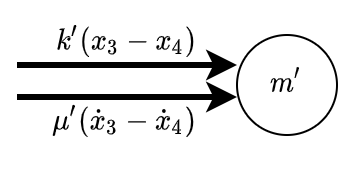
\includegraphics[width=\textwidth]{Percussion1D3-Masse4}}
                \end{subfigure}
                   \caption{Bilan des forces}
            \end{figure}

            \vspace*{-0.5cm}
            \myfigframe{Percussion1D3-Apres.png}{Situation \textcolor{red}{après} contact}

        }

        % \pause
        \mycol{50}{
            Le système est régi par les équations :
            \begin{align*}
                \begin{dcases}
                m\ddot x_1 = -k(x_1 - x_2) - \mu (\dot x_1 - \dot x_2) \,, \\
                m\ddot x_2 = k(x_1 - x_2) + \mu (\dot x_1 - \dot x_2) - \textcolor{red}{F_c} \,, \\
                m'\ddot x_3 = - k'(x_3 - x_4) - \mu'(\dot x_3 - \dot x_4) + \textcolor{red}{F_c} \,, \\
                    m' \ddot x_4 =  k'(x_3 - x_4) + \mu'(\dot x_3 - \dot x_4) \,. 
                \end{dcases}
            \end{align*}

            \pause
            Avec $\varepsilon$ est le coefficient de restitution et :
            \scriptsize
            $$
            I = \int_{\tmoins}^{\tplus} k(x_1 - x_2) + \mu (\dot x_1 - \dot x_2) - k'(x_3 - x_4) - \mu'(\dot x_3 - \dot x_4) \diff t \,,
            $$
            \normalsize
            les vitesses après contact sont :
            \begingroup
            \color{red}
            \begin{align*}
                V_0 = \frac{I + (m-\varepsilon m')v_0 + (1+\varepsilon)m'v'_0}{m+m'}\,, \\
                V'_0 = \frac{I + (1+\varepsilon)mv_0 + (m'-\varepsilon m)v'_0}{m+m'}\,.
            \end{align*}
            \endgroup
            
            \note{Le calcul des vitesses ici était notre première tentative de trouver ce qui se passe véritablement après un contact. Nous avons complexifier les choses par la suite.}

        }

    }
    
\end{frame}




\begin{frame}{Des modèles généraux pour la percussion avec séparation des masses (1)}

	\myfigframesize{Deplacement1D-2.png}{Illustration d'un floe 1D contenant $n$ masses}{80}
	
	\small
	\vspace*{-0.1cm}
	Sous forme matricielle, on a le système:
	\begin{align} \label{eq:percussion1d4}
    \begin{pmatrix}
        \dot z_0 \\ \dot z_1 \\ \vdots \\ \dot z_{n-1} \\ \ddot z_0 \\ \ddot z_1 \\ \vdots \\ \ddot z_{n-1}
    \end{pmatrix}
    = 
    \frac{1}{m} \underbrace{\begin{pmatrix}
        \begin{matrix}
       & & &  \\ & & &  \\ & & \bigzero & \\ & & & \\      
        \end{matrix}
        & \rvline 
        & \begin{matrix}
        & & & \\ & & &  \\ & I_n & & \\ & & & \\
        \end{matrix}  \\ 
        \hline
        \begin{matrix}
            & & &  \\ & & B & \\ & & & \\ & & & \\     
        \end{matrix}
        & \rvline 
        &\begin{matrix}
            & & & \\ & C & & \\ & & & \\ & & & \\        
        \end{matrix}
      \end{pmatrix}}_{2n \times 2n}
      \begin{pmatrix}
        z_0 \\ z_1 \\ \vdots \\ z_{n-1} \\ \dot z_0 \\ \dot z_1 \\ \vdots \\ \dot z_{n-1}
        \end{pmatrix}
    +
    \frac{1}{m} \underbrace{\begin{pmatrix}
        \begin{matrix}
       & & &  \\ & & &  \\ & & \bigzero & \\ & & & \\      
        \end{matrix}
        & \rvline 
        &     \begin{matrix}
            & & &  \\ & & &  \\ & \bigzero & & \\ & & & \\      
             \end{matrix}  \\ 
        \hline
        \begin{matrix}
            & & &  \\ & & D & \\ & & & \\ & & & \\     
        \end{matrix}
        & \rvline 
        &   \begin{matrix}
            & & &  \\ & \bigzero & &  \\ & &  & \\ & & & \\      
            \end{matrix}
      \end{pmatrix}}_{(2n) \times (2n-2)}
      \begin{pmatrix}
        L0_0 \\ L0_1 \\ \vdots \\ L0_{n-2} \\ 0 \\ 0 \\ \vdots \\ 0
        \end{pmatrix} \,,
	\end{align}
	
	où:
	\scriptsize
	$$
B =  \begin{pmatrix}
    -k & k &  &  &  \\
    k & -2k & k &  &  \\
     & \ddots & \ddots & \ddots &  \\
     &  & k & -2k & k \\
     &  &  & k & -k
    \end{pmatrix} , 
C =  \begin{pmatrix}
    -\mu & \mu &  &  &  \\
    \mu & -2\mu & \mu &  &  \\
     & \ddots & \ddots & \ddots &  \\
     &  & \mu & -2\mu & \mu \\
     &  &  & \mu & -\mu
    \end{pmatrix} , 
D =  \begin{pmatrix}
    -k &  &  &  \\
    k & -k &  &  \\
     & \ddots & \ddots &  \\
     &  & \ddots & -k \\
     &  &  & k 
    \end{pmatrix}.
	$$
    \normalsize

    \note{On commence à utiliser z ici et non x parce que (pour une raison inexpliquée), les longueurs à vide des ressorts ne sont pas respectées.}
\end{frame}


\begin{frame}{Des modèles généraux pour la percussion avec séparation des masses (2)}

\begin{figure}[!h]
    \begin{subfigure}[b]{0.30\textwidth}
        \centering
        \frame{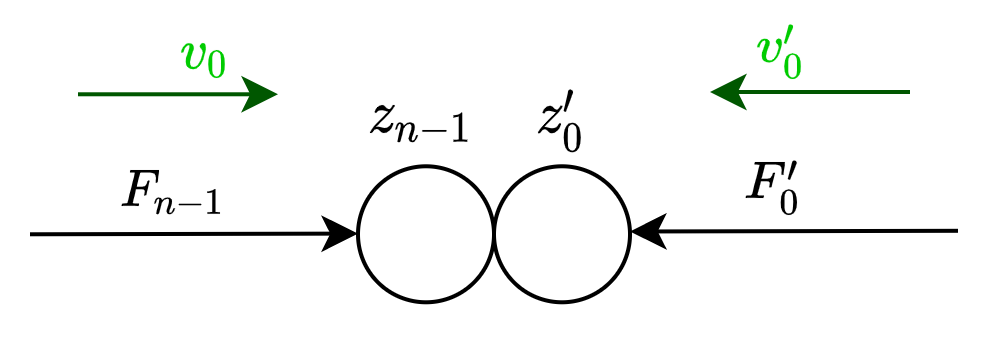
\includegraphics[width=\textwidth]{Percussion1D-4-Avant.png}}
        \caption{Avant le choc}
    \end{subfigure}
%     \hfill
    \begin{subfigure}[b]{0.29\textwidth}
        \centering
        \frame{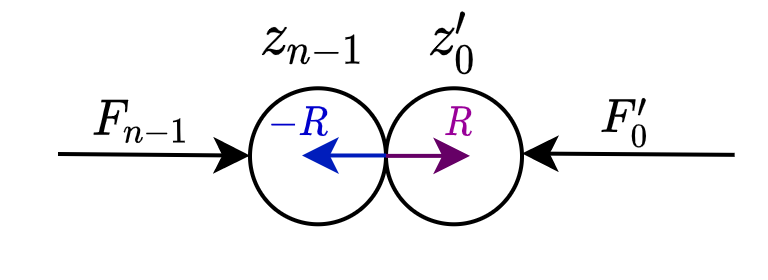
\includegraphics[width=\textwidth]{Percussion1D-5.png}}
        \caption{Pendant le choc}
    \end{subfigure}
    \begin{subfigure}[b]{0.30\textwidth}
        \centering
        \frame{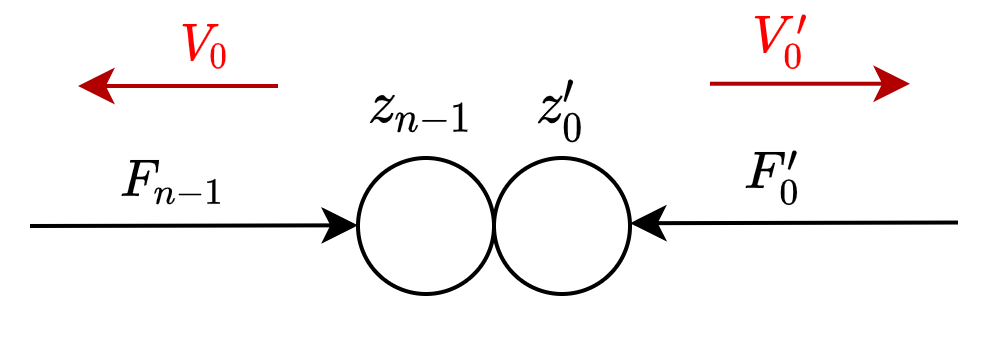
\includegraphics[width=\textwidth]{Percussion1D-4-Apres.png}}
        \caption{Après le choc}
    \end{subfigure}
\end{figure}


%\myfigframesize{Percussion1D-4-Avant.png}{Avant le choc}{40}
%\myfigframesize{Percussion1D-4-Apres.png}{Après le choc}{40}


	\mycols{
		\mycol{50}{	
        \begin{alertblock}{Un modèle qui conserve l'énergie cinétique après chaque choc.}
        \begin{align}
			\textcolor{red}{V_0 = \frac{-b \pm \sqrt{\Delta}}{2a}, \quad V'_0 = V_0 + X\,,}
		\end{align}
		avec :
		\begin{align*}
		X = \varepsilon(v_0 - v'_0)&, \, Y = m(v_0)^2 + m'(v'_0)^2\,,\\  a &= m+m'\,,\\ b &= -2m'X\,,\\ c &= m'X^2 - Y \,,\\ \Delta &= b^2 - 4ac.
		\end{align*}
		\end{alertblock}
		}
		
        \pause
		\mycol{50}{	
        \begin{exampleblock}{Un modèle qui met en évidence le coefficient de restitution \parencite{hecker1997collision}.}
		\begin{align} \label{eq:perc5eq2}
            \textcolor{red}{V_0 = v_0 + \frac{J-I}{m} , \quad
        V'_0 = v'_0 + \frac{K+I}{m'}\,,}
		\end{align}
		avec:
		\begin{align*}
        I = \frac{(v_0 - v'_0)(1+\varepsilon) +\frac{J}{m} - \frac{K}{m'}}{\frac{1}{m}+\frac{1}{m'}}, \\
    		J = \int_{t^{-}}^{t^{+}} F_{n-1} \diff t = F_{n-1} \, \Delta t, \\ 
    		K = \int_{t^{-}}^{t^{+}} F'_{0} \diff t = F'_{0} \, \Delta t.
		\end{align*}

		\end{exampleblock}
		}
		
		\note{Technique répandue dans le monde du jeux vidéo pour le codage des graphics engines!!}

	}
\end{frame}



\begin{frame}{Des modèles généraux pour la percussion avec séparation des masses (3)}

	\myfig{Screenshot1.jpg}{Configuration des floes pour la simulation}

	\mycols{
		\mycol{50}{	
        % \begin{alertblock}{\vspace*{-0.5cm}}
        \begin{alertblock}{Premier modèle généralisant}
		\myfig{EnsPlotPerc2.png}{Résultat pour le modèle qui conserve l'énergie cinétique après chaque choc}
		\vspace*{-0.2cm}
		\end{alertblock}
		}
		
        \pause
		\mycol{50}{	
        % \begin{exampleblock}{\vspace*{-0.5cm}}
        \begin{exampleblock}{Deuxième modèle généralisant}
		\myfig{EnsPlotPerc3.png}{Résultat pour le modèle qui met en évidence le coefficient de restitution}
		\vspace*{-0.2cm}
		\end{exampleblock}
		}
		
		\note{Technique répandue dans le monde du jeux vidéo pour le codage des graphics engines!!}

	}
    \note{Vu que je n'ai toujours rien décider pour le modèle final, c'est mieux de dire qu'*on ne peut pas tout avoir*. La conservation de l'énergie (au niveau macroscopique) dépend de ce qui se passe entre les deux noeuds concernés pendant la percussion (niveau microscopique).
    }
\end{frame}









\subsection{Fracturation des floes}


\begin{frame}{Différents modèles de fracture fragile}

% \vspace{-0.5cm}
\myfigsize{PhaseFieldExplainer.png}{Champ de phase pour la régularisation d'une fissure \parencite{yvonnet2018fissuration}}{65}
% \vspace{-0.5cm}
	
	\mycols{
		\mycol{45}{	
        \begin{exampleblock}{Méthode du champ de phase}
        % \vspace{-0.4cm}
        \small
        \begin{align*}
            E = \int_{\Omega} \Psi(\bvec{u},\Gamma) &\diff\Omega + G_c\int_{\Gamma} \diff \Gamma, \\
        &\big\Downarrow \\
            E = \int_{\Omega} \Psi(\bvec{u},\Gamma) \diff\Omega &+ G_c\int_{\Gamma} \textcolor{orange}{\gamma(d, \nabla d)} \diff \Gamma.
        \end{align*}
		%  \vspace{-0.2cm} 
		\end{exampleblock}
		}

        \pause

		\normalsize
		\mycol{55}{	
        \begin{alertblock}{Méthode combinatoire}
            \begin{align*} \label{eq:modelcombi}
                E^{n+1} & = \text{eng. pot. élastique au temps } t^{n+1}  \\
                & + \text{ ténacité}\times \text{lg. de la fracture envisagée à }t^{n+1}.  
            \end{align*}
		% \vspace*{0.001cm} 
		\end{alertblock}
		}

	}
	% \vspace{0.2cm}

    \note{Pour le modèle combinatoire, bien préciser qu'on est en déformation élastique: et donc la longueur de la fracture est la longueur initiale des ressorts. Si les d;eplacements étaient plasiqques, ca ne serait pas la même chose.}

\end{frame}


\begin{frame}[fragile]{Code de calcul 1D}

	\centering
    \textcolor{mygray}{\href{run:../../../../Share/FracSimu.gif}{\textbf{Animation de la fracture 1D par un algorithme \emph{event-driven}}}}

    % \only<2>{
	\animategraphics[loop,controls,autoplay,width=\linewidth]{10}{Simu1D/FracSimu-}{0}{312}
    % }

    \tiny
    \begin{lstlisting}[language=Python,breaklines,caption={Code de simulation 1D},captionpos=b,label={code}]
        def runSimulation(self):
            """
            Runs the simulation for the complete fracture problem
            """
    
            ## Run uniform mouvement phase up to the first collision
            self.computeBeforeContact()
    
            for key in self.floes.keys():
                self.checkFracFrom[key] = self.t.size
    
            while self.t.size <= self.NBef + self.NAft and max(self.collCount.values()) < 1000:
    
                self.computeAfterContact()
    
                ## (Potential) fracture detection 
                floeDict = deepcopy(self.floes)
                for floe in floeDict.values():
                    self.checkFracture(floe.id)
    
                ## Collision detection 
                for floe in self.floes.values():
                    for node in floe.nodes:
                        res = self.checkCollision(node.id, node.rightNode)
    
                ## Assign the same value to all keys to check collision from now on
                smallestCheckCollFrom = min(self.checkCollFrom.values())
                for key in self.checkCollFrom.keys():
                    self.checkCollFrom[key] = smallestCheckCollFrom
    
                ## Assign the same value to all keys tp check fracture from now on
                smallestCheckFracFrom = min(self.checkFracFrom.values())
                for key in self.checkFracFrom.keys():
                    self.checkFracFrom[key] = min([smallestCheckFracFrom, smallestCheckCollFrom])
    \end{lstlisting}
    \normalsize

\end{frame}
    
    



% 
%-------------------------------------------------------------------------------
%							FOURTH SECTION
%-------------------------------------------------------------------------------


\section{\textsc{Travaux 2D}}


\subsection{Déplacement des n\oe{}uds}


\begin{frame}{Déplacement des n\oe{}uds d'un floe isolé (1)}

    \mycols{

        \mycol{40}{

            \begin{figure}
                \centering
                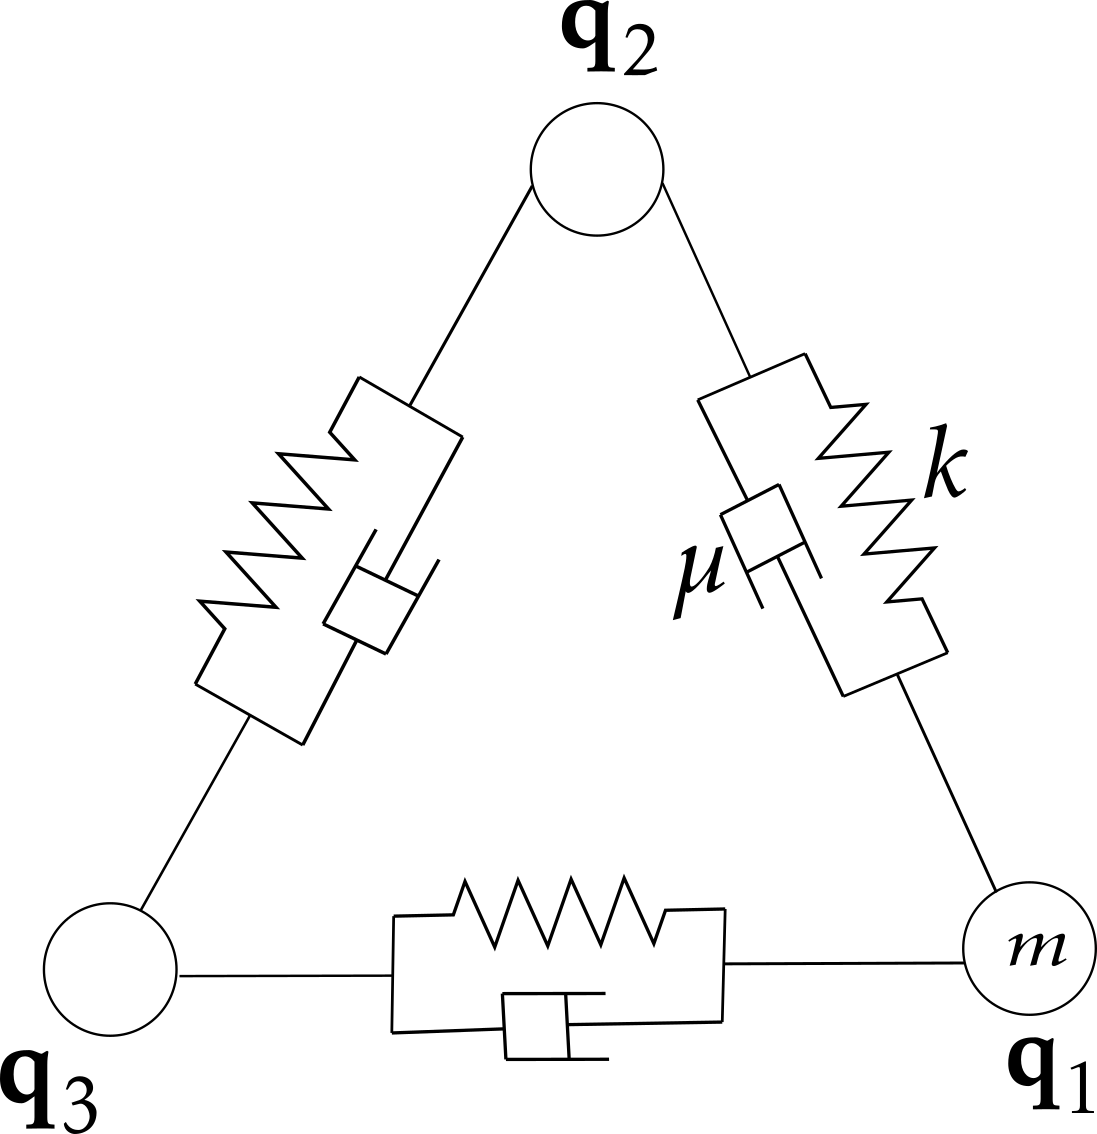
\includegraphics[width=0.6\textwidth]{Deplacement2D-1.png}
                \caption{Floe de glace 2D \vspace{0.5cm}}
            \end{figure}

        }

        \mycol{60}{
            % \onslide<2>{\myfig{PlotDeplacement2D-1-NonConv.png}{Simulation avec $T=10$}}

            \begin{figure}
                \centering
                \includegraphics<2>[width=\textwidth]{PlotDeplacement2D-1-NonConv.png}
                \onslide<2>{\caption{Simulation avec $T=10$} \vspace{-0.5cm}}
            \end{figure}
            % \myfig{PositionInitFinales.png}{Illustration à $T=4$}
        }

    }

	% \onslide<1>{\vspace{0.5cm}}

	% \onslide<2>{\vspace{-1cm}}
    Les équations de Newton-Euler :
    \begin{align*}
        \forall i \in \mathbb{Z}/3\mathbb{Z}, \quad m \ddot{\bvec{q}}_i = \underbrace{\sum_{j=i+1}^{i+2} \textcolor{teal}{C_{ij}} \left[  \textcolor{blue}{k \left( \Vert \bvec{q}_j - \bvec{q}_i \Vert - L_{ij} \right) \bvec{u}_{ij}} \textcolor{orange}{- \mu \left\langle \dot{\bvec{q}}_j - \dot{\bvec{q}}_i, \, \bvec{u}_{ij}  \right\rangle  \bvec{u}_{ij}}  \right]}_{\bvec F_i} . 
    \end{align*}

    Schéma d’Euler explicite :
    \begin{align*}
        \bvec{q}_{i}^{n+1} = 2\bvec{q}_{i}^{n}-\bvec{q}_{i}^{n-1} + \frac{\Delta t^2}{m} \sum_{j=i+1}^{i+2}C_{ij}\left[ k \left( \Vert \bvec{q}_j^n - \bvec{q}_i^n \Vert - L_{ij} \right) \bvec{u}_{ij} - \frac{\mu}{\Delta t} \left\langle \bvec{q}_{j}^{n}-\bvec{q}_{j}^{n-1} - \bvec{q}_{i}^{n}+\bvec{q}_{i}^{n-1}, \, \bvec{u}_{ij} \right\rangle  \bvec{u}_{ij}  \right].
    \end{align*}
    
\end{frame}


\begin{frame}[fragile]{Déplacement des n\oe{}uds d'un floe isolé (2)}

    \tiny
    \begin{lstlisting}[language=Python,caption=Code de simulation et schéma avec Scipy]
                                    q0 = np.stack([q1_0, dotq1_0, q2_0, dotq2_0, q3_0, dotq3_0])
                                    q0_ = np.reshape(q0, (nb_nodes*4))

                                    def model(t, Q_):
                                        Q = np.reshape(Q_, (nb_nodes*2, 2))
                                        Q_ret = np.zeros_like(Q)
                                        Q_ret[2*0] = 0; Q_ret[2*1] = 0
                                        
                                        for i in range(1, nb_nodes):  ## <-- Node 0 is immobilized
                                            Q_ret[2*i] = Q[2*i+1] 
                                            
                                            for neighbor in range(i+1, i+3):
                                                j = neighbor % nb_nodes
                                                u[i,j] = (Q[2*j] - Q[2*i]) / nplin.norm(Q[2*j] - Q[2*i])
                                                Q_ret[2*i+1] += (1 / m)*C[i,j]*( k*(nplin.norm(Q[2*j]-Q[2*i]) - L[i,j])*u[i,j]
                                                                -  mu*(np.dot(Q[2*j+1] - Q[2*i+1], u[i,j]))*u[i,j] )
                                        return np.reshape(Q_ret, (nb_nodes*4))

                                    sol = solve_ivp(model, [0,T], q0_, t_eval=t)
    \end{lstlisting}
    
	\hspace*{-1cm}
	\mycols{
	
	\mycol{70}{
	    \begin{figure}
        \centering
        \hspace{-1cm}
        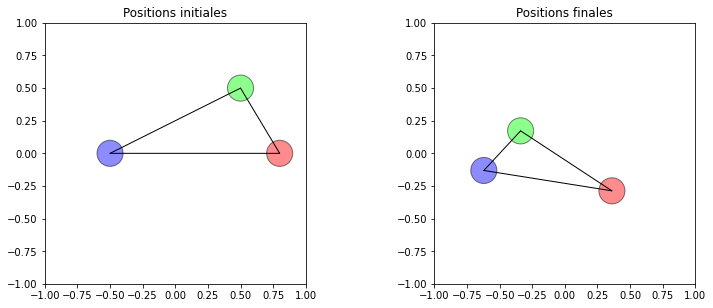
\includegraphics[width=0.8\textwidth]{PositionInitFinales.png}
        %\hspace{-1.5cm}
        \caption{Illustration à $t=0$ et $t=4$}
    	\end{figure}
	}
	
	\hspace{-0.5cm}
	
	
	\mycol{32}{

	% \vspace{-0.5cm}
	% \normalsize
	% \hspace{-1cm}
	% \begin{adjustwidth}{1cm}{2cm}
	%    \begin{alertblock}{En somme}
    %      Avec un schéma Euler explicite, symplectique ou Scipy (RK45), il faut fixer certains n\oe{}uds pour que le système reste stable!
    %     \end{alertblock}
	% \end{adjustwidth}	

    \scriptsize
    \begin{tcolorbox}[colback=red!5,colframe=red!50!black,arc=0mm,boxrule=0.1mm,title=Observation]
        \vspace*{-0.1cm}
            Avec un schéma Euler explicite, symplectique ou Scipy (RK45), il faut fixer certains n\oe{}uds pour que le système reste stable!
        \vspace*{-0.1cm}
    \end{tcolorbox}

	}	
	\normalsize
	}
	

\end{frame}




\subsection{Percussion entre floes}


\begin{frame}{Collision parfaitement inélastique entre deux floes (1)}

    \mycols{

        \mycol{40}{
			\myfigframe{Percussion2DNew.png}{Illustration de la percussion 2D}

\begin{align*}
\begin{dcases}
    (m+m') \ddot{\bvec{q}}_0  = \bvec{F}_0 + \bvec{F}^{'}_0  , & \textcolor{cyan}{\text{(SE)}} \\
    \ddot{\bvec{p}}_0 = \ddot{\bvec{q}}_0 , \dot{\bvec{p}}_0 = \dot{\bvec{q}}_0 , \bvec{p}_0 = \bvec{q}_0 - \Delta_0 , & \textcolor{cyan}{\text{(SE)}} \\
    m \ddot{\bvec{q}}_i = \bvec{F}_i   \,, \quad \quad \quad \forall 1 \leq i \leq n-1 , & \textcolor{orange}{\text{(SI)}} \\
    m' \ddot{\bvec{p}}_i = \bvec{F}^{'}_i   \,, \quad \quad \quad \forall 1 \leq i \leq n'-1 , & \textcolor{orange}{\text{(SI)}}
\end{dcases}
\end{align*}
où : $\quad \Delta_0 = \bvec{q}_0(0) - \bvec{p}_0(0)$.
			
        }

        \pause
        \mycol{60}{
            \myfigframesize{Percussion2DSlides}{Un maillage 2D par processus de Poisson}{80}
            
            \centering
    \textcolor{mygray}{\href{run:../../../../Share/ShortAnim2D.gif}{\textbf{Animation de la percussion 2D}}}

		\animategraphics[loop,controls,autoplay,width=\linewidth]{10}{Simu2D/ShortAnim2D-}{0}{70}
	
        }

    }
    
\end{frame}




\begin{frame}{Collision parfaitement inélastique entre deux floes (2)}

	\myfigframesize{ClientWebMoi.jpg}{Client web développé et maintenu avec Flask}{60}
	\note{En fin je dois vous montrer ce clien web.  Je ne pouvais m'en empécher.}
    
\end{frame}


% 
%-------------------------------------------------------------------------------
%							FITH SECTION
%-------------------------------------------------------------------------------

\section{\textsc{Conclusion}}


\subsection{Bilan}

\setbeamercovered{transparent}
\begin{frame}{Apports et recherches ultérieures}

    \vspace{-0.2cm}
	\myfigsize{Timeline}{Résumé du déroulement du stage}{65}
	\note{Prendant la soutenance, et dans le rapport, il faut dire que j'ai utilisé une méthode Agile. Plus précisément Scrum. Même si cela n'était aps très formel, j'implémentais une fonctionnalité chaque semaine; sauf que pour le dernier mois de stage, il a fallut coder un gros truc.. }

	\note{On a commencer par la lecture des travaux antérieus, et on a fini par la percussion 1D en pasant par la percussion 2D. Ca semble contre-intuitif MAIS c'est nécésssaire pour avancer.}
	\pause
	\small
	
    \vspace{-0.3cm}
	\mycols{	
		
		\mycol{50}{
        \begin{alertblock}{Recherches ultérieures}
        \begin{itemize}
        \item Implémentation de la méthode du champ de phase;
        \item Implementation de la fracture au problème 2D, 2.5D, ou 3D;
        \item Intégration de la fracture au code de \citeauthor{rabatel2015modelisation};
        \item Confirmation de l'approximation par réseaux de ressorts;
        \item Optimiser les codes avec Cython ou en C++;
        \item Tests de validation en laboratoire.
        \end{itemize}
		\end{alertblock}
		}

        \pause
        \note{Pour le passage en dimension supérieure, mentionner le CoD Curse of Dimensionnalyty qui s'est posé lorsque je suis passé de la 1D à la 2D, et qui se passera en passant à la 3D}


		\mycol{50}{
        \begin{exampleblock}{Apports du stage}
        \begin{itemize}[<+->]
        \item Simulation de systèmes dynamiques en Python;
        \item Prise en main du modèle de rupture de Griffith (analyse fonctionnelle, analyse numérique, etc.);
        \item Maitrise de l'approche par réseaux de ressorts (probabilité, raisonnance);
        \item Utilisation de TikZ, Flask, Bokeh, Symbolab, et bien d'autres;
        \item Recherche en milieu professionnel;
        \item Savoir-faire transférables (vision globale, etc.).
        \end{itemize}
		\end{exampleblock}
		}
        
        \note{Blague sur TikZ: La loi de Murphy. Etant donné assez de temps, tout peut arriver. C'est comme ca j'ai apris TIKZ, en 6 mois !!}

		
	}
    
\end{frame}




\subsection{Délivrables}

\begin{frame}{Liste récapitulative et délivrables}

        \begin{block}{Checklist des objectifs}
    	\begin{enumerate}
      	\item[\checkmark] Prise en main de la notion de $\Gamma$‑convergence; \pause
      	\item[\checkmark] Assimilation des travaux antérieurs; \pause
      	\item[\checkmark] Modélisation de la percussion (1D et 2D); \pause
      	\item[\checkmark] Modélisation de la fracture: 
      	\begin{itemize}
        \item[\checkmark] en 1D;
        \item[$\times$] en 2D. 
        \end{itemize} \pause
      	\item[$\times$] Calculs à l'échelle des floes de glace de l'Arctique. \pause
      	\end{enumerate}
		\end{block}
	
        \setbeamercovered{invisible}
        \pause
        \begin{exampleblock}{Délivrables}
        \begin{enumerate}
        \item Rapport de stage: \myemoji \textcolor{orange}{\href{https://github.com/desmond-rn/ice-floes/tree/master/pdf}{ GitHub}};
        \item Code de calcul: \myemoji \textcolor{orange}{\href{https://github.com/desmond-rn/ice-floes/tree/master/code}{ GitHub}} et \myemoji \textcolor{orange}{\href{https://framagit.org/RaK/SimuRessorts}{ Framagit}};
        \item Quelques simulations: \myemoji \textcolor{orange}{\href{https://seafile.unistra.fr/d/a6c3680909624b22be7c/}{ Seafile}}.
        \end{enumerate}
		\end{exampleblock}
    
\end{frame}




% %-------------------------------------------------------------------------------
% %							THE BIBLIOGRAPHY
% %-------------------------------------------------------------------------------

\appendix   % Pour retirer les references de la bare de navigation
% \vspace*{0.5mm}


% \hspace*{-0.75cm}\parbox[t]{\textwidth} 

\tiny
\printbibliography

% %-------------------------------------------------------------------------------
% %							THANK YOU NOTE 
% %-------------------------------------------------------------------------------

  \begin{frame}
    \Large
    \begin{exampleblock}{\centering \LARGE Thank you for your kind attention \Large \Smiley{} !}\LARGE
      \centering
      Questions ?
    \end{exampleblock}

  \end{frame}


\end{document}

